\textbf{Цель работы:} изучение принципов построения, функционирования и программирования магистрально-модульной аппаратуры КАМАК на примере программно-аппаратной реализации устройства динамической индикации (\enquote{часы-будильник}) с использованием 6 семисегментных светодиодных индикаторов.

\textbf{Аппаратура:} лабораторный макет устройства динамической индикации, источник питания $+7.5..9\textrm{В}$, аппаратура КАМАК (входной регистр 305, выходной регистр 350), соединительный кабель.

\section{Минимальные теоретические сведения}

\subsection{Описание лабораторного макета}

Устройство индикации, используемое в лабораторной работе, частично содержит функциональные элементы, необходимые для организации режима динамической индикации.

В состав устройства входят:

\begin{enumerate}
\item Тактовый генератор
\item Счетчик адреса
\item Дешифратор адреса
\item Транзисторные ключи включения разрядов и формирователи тока семисегментных индикаторов
\item Два трехразрядных семисегментных светодиодных индикатора ТОТ3361АН с общими катодами
\item Формирователь звукового сигнала
\end{enumerate}

Остальные устройства должны быть реализованы программно-аппаратным образом с использованием аппаратуры КАМАК -- входного регистра 305 и выходного регистра 350.

Устройство формирует 3-х разрядный код адреса, который выдается на внешний разъем (на входной регистр 305) и одновременно поступает на внутренний дешифратор адреса. Дешифратор управляет транзисторными ключами, поочередно подключая катоды 6-и семисегментных индикаторов к общему проводу (земле) источника питания. Информация на сегменты индикатора должна поступать из внешнего устройства (выходной регистр 350) синхронно с кодом адреса соответствующего разряда индикатора.

На входной регистр 305 также поступают сигналы нажатия кнопки \enquote{индикация будильника} и включения тумблера \enquote{сигнал}, предназначенные для реализации устройством функций будильника. Сигнал управления включением будильника на устройство динамической индикации поступает с выходного регистра 350.



\section{Результаты и их обсуждение}

\subsection{Интерфейс программы управления}

Для организации непрерывного управления устройством была разработана программа с графическим интерфейсом (\autoref{fig:app}).

\begin{figure}[h]%
\centering
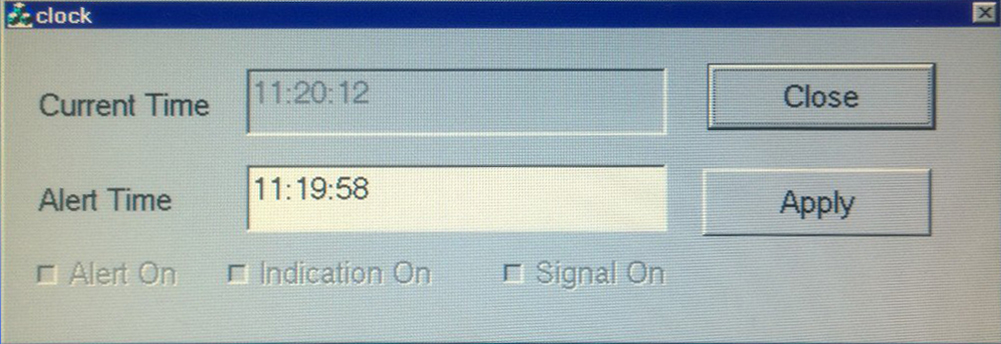
\includegraphics[width=0.8\textwidth]{app}%
\caption[Главное окно программы.]{Главное окно программы}%
\label{fig:app}%
\end{figure}

Индикаторы (флажки) показывают текущее состояние аппаратуры (тумблер \enquote{сигнал} взведен, кнопка \enquote{индикация будильника} нажата, звуковой сигнал включен).

В двух текстовых полях отображаются текущее время и время срабатывания будильника. Рядом с последним имеется кнопка для применения новой настройки будильника.

\subsection{Архитектура программы управления}

Для обеспечения непрерывной индикации времени работа с аппаратурой КАМАК через программный интерфейс аппаратуры производится из отдельного фонового потока.

Класс, инкапсулирующий работу с аппаратурой, содержит поля для хранения текущего времени и времени срабатывания будильника, а также функции-члены для потокобезопасного доступа к ним. Главный поток приложения (поток управления пользовательским интерфейсом) содержит код управления жизненным циклом класса, а так же по таймеру с интервалом в несколько сотен миллисекунд обновляет его поля.

Фоновый поток

\begin{enumerate}[label=\asbuk*)]

\item непрерывно считывает значения полей (текущее время, время срабатывания будильника) и содержимое регистра 305 с шины магистрали КАМАК (трехразрядный код адреса, состояние тумблера \enquote{сигнал} и кнопки \enquote{индикация будильника}),

\item в зависимости от кода адреса выдает в выходной регистр код цифры одного из временн\'{ы}х разрядов текущего времени или времени срабатывания будильника в зависимости от состояния кнопки \enquote{индикация будильника} (код адреса соответствует одному из шести семисегментных индикаторов из блока индикаторов) или сигнал состояния индикатора включения будильника (код адреса соответствует индикатору включения будильника),

\item выдает звуковой сигнал при попадании текущего времени в интервал времени сигнализации будильника (60 секунд считая от времени срабатывания будильника),

\item выдает в главный поток информацию об изменениях в состоянии аппаратуры через функцию обратной связи и механизм сообщений Windows

\end{enumerate}

\section{Выводы}

В ходе работы была реализована программа управления устройствами магистрально-модульной аппаратурой КАМАК на примере программно-аппаратного комплекса динамической индикации \enquote{часы-будильник}.

Были изучены принципы построения, функционирования и программирования магистрально-модульной аппаратуры КАМАК.